% !TEX root = ../TAMU_Thesis_Main.tex
%%%%%%%%%%%%%%%%%%%%%%%%%%%%%%%%%%%%%%%%%%%%%%%%%%%%%%%%%%%%%%%%%%%%%%%
%%%                           Chapter II
%%%%%%%%%%%%%%%%%%%%%%%%%%%%%%%%%%%%%%%%%%%%%%%%%%%%%%%%%%%%%%%%%%%%%%

\Chapter{Literature Review: The Importance of Research Part Two- This is designed to test long titles in the TOC}

Text goes here.

\section{New Section}
%%%%%%%%%%%%%%%%%%%%%%%%%%%%%%%%%%%%%%%%%%%%%%%%%%%%%%

\lipsum[1-3]

\begin{figure}[!h]
	\centering
	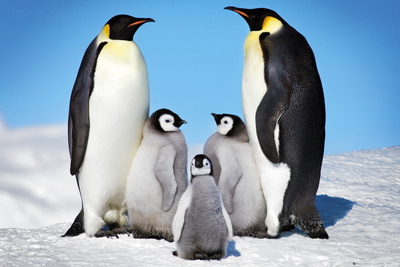
\includegraphics[width=0.5\textwidth]{./Figures/Penguins.jpg}
	\caption{TAMU figure - This is an example of a long figure title.  Figure titles need to be single-spaced within and double spaced between in the list of figures.}
	\label{fig:landscapepenguins}
\end{figure}

\lipsum[4]
%%%%%%%%%%%%%%%%%%%%%%%%%%%%%%%%%%%%%%%%%%%%%%%%%%%%%%
\subsection{Subsection}
\begin{table}[H]
\centering
\caption{This is a table template - This is an example of a long table title.  Table titles need to be single-spaced within and double spaced between in the list of tables.}
\begin{tabular}{|l|c|c|c|c|c|}
\hline
Product & 1 & 2 & 3 & 4 & 5\\
\hline
Price & 124.- & 136.- & 85.- & 156.- & 23.-\\
Guarantee [years] & 1 & 2 & - & 3 & 1\\
Rating & 89\% & 84\% & 51\% & & 45\%\\
\hline
\hline
Recommended & yes & yes & no & no & no\\
\hline
\end{tabular}
\label{tab:template1}
\end{table}


\subsection{Subsection}
%%%%%%%%%%%%%%%%%%%%%%%%%%%%%%%%%%%%%%%%%%%%%%%%%%%%%%
\begin{figure}[H]
\centering
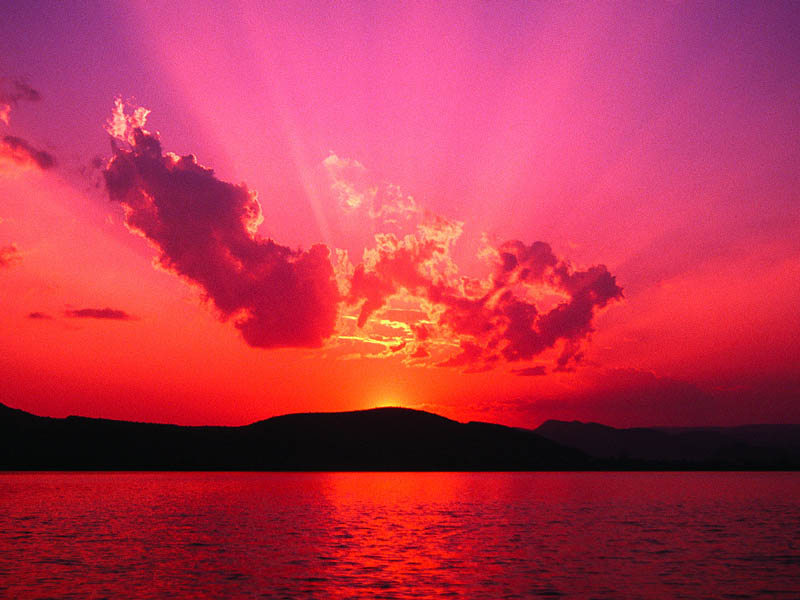
\includegraphics[scale=.50]{figures/Sunset.jpg}
\caption{Sunset figure}
\label{fig:sunset-fig2}
\end{figure}
%%%%%%%%%%%%%%%%%%%%%%%%%%%%%%%%%%%%%%%%%%%%%%%%%%%%%%
\subsubsection{This is a subsubsection}
\begin{table}[H]
\centering
\caption{This is a table template - This is an example of a long table title.  Table titles need to be single-spaced within and double spaced between in the list of tables.}
\begin{tabular}{|l|c|c|c|c|c|}
\hline
Product & 1 & 2 & 3 & 4 & 5\\
\hline
Price & 124.- & 136.- & 85.- & 156.- & 23.-\\
Guarantee [years] & 1 & 2 & - & 3 & 1\\
Rating & 89\% & 84\% & 51\% & & 45\%\\
\hline
\hline
Recommended & yes & yes & no & no & no\\
\hline
\end{tabular}
\label{tab:template1-2}
\end{table}
\section{Another Section}
